\Opensolutionfile{ans}[ans/ans-on-tap-chuong-4]
%Câu 1
\begin{ex}%[1K4YD-1]
	Phát biểu nào sau đây là \textbf{sai}?
	\choice
	{Hình biểu diễn của một đường tròn có thể là một elip}
	{\True Hình biểu diễn của một hình thang (không phải là hình bình hành) có thể là một hình bình hành}
	{Hình biểu diễn của một tam giác đều có thể là một tam giác}
	{Hình biểu diễn của một hình vuông có thể là một hình bình hành}
	\loigiai{
		Hình biểu diễn của một hình không gian là hình chiếu song song của nó lên một mặt phẳng theo một phương chiếu nào đó. Do đó hình biểu diễn của hai đường thẳng cắt nhau là hai đường thẳng cắt nhau. Vậy phát biểu ``Hình biểu diễn của một hình thang (không phải là hình bình hành) có thể là một hình bình hành'' là sai.
	}
\end{ex}
%Câu 2
\begin{ex}%[1K4YB-1]
	Cho hai đường thẳng $a$, $b$ chéo nhau. Có bao nhiêu mặt phẳng chứa $a$ song song với $b$?
	\choice
	{\True $1$}
	{$0$}
	{$2$}
	{Vô số}
	\loigiai{
	Có duy nhất một mặt phẳng chứa $a$ và song song với $b$ vì có duy nhất một mặt phẳng chứa hai đường thẳng cắt nhau.
	}
\end{ex}
%Câu 3
\begin{ex}%[1K4B0-3]
	Cho hình chóp $S.ABCD$, đáy là hình thang, đáy lớn $AB$, giao tuyến của mặt $(SAD)$ và $(SBC)$ là
	\choice
	{ $Sx$ với $Sx \parallel AB$}
	{$SK$ với $K=AC\cap BD$}
	{\True $SK$ với $K=AD \cap BC$}
	{$SK$ với $K=AB \cap CD$}
	\loigiai{
		\immini{
			Kéo dài $AD$ và $BC$. Gọi $K$ là giao điểm của $AD$ và $BC$.\\
			Ta có $S$ và $K$ là hai điểm chung của hai mặt phẳng $(SAD)$ và $(SBC)$ nên giao tuyến của $(SAD)$ và $(SBC)$ là $SK$.
		}
		{
		\begin{tikzpicture}[scale=1, line join = round, line cap = round]
			\tikzset{declare function={a=4;b=2;h=5;goc=-60;}}
			\draw
			(0,0)coordinate (A)+(0:a)coordinate (B)
			(goc:b)coordinate (D)+(70:h)coordinate (S) ($(B)+(D)-(A)$)coordinate (c)
			($(c)!.6!(D)$)coordinate (C)
			(intersection of A--D and B--C)coordinate (K)
			;
			\foreach \pointo/\pointt in {B/C,D/A,S/A,S/B,S/C,S/D,S/K,C/K,D/K}{
				\draw[fill=black](\pointo)--(\pointt);
			}
			\foreach \pointo/\pointt in {A/B,C/D}{
				\draw[fill=black,dashed](\pointo)--(\pointt);
			}
			\foreach \point/\goc in {S/90,A/190,B/-10,C/-10,D/190,K/-90}{
				\draw[fill=black](\point)circle(1pt)+(\goc:2.5mm)node[scale=.8]{$\point$};
			}
		\end{tikzpicture}
		}
	}
\end{ex}
%Câu 4
\begin{ex}%[1K4BB-3]
	Cho hình chóp $ S.ABCD $ có đáy $ ABCD $ là hình bình hành. Gọi $ I,J $ lần lượt là trung điểm của $ AB $ và $ CD $. Giao tuyến của hai mặt phẳng $ (SAB) $ và $ (SCD) $ là đường thẳng song song với đường thẳng nào sau đây?
	\choice
	{$IJ$}
	{\True$BI$}
	{$BJ$}
	{$AD$}
	\loigiai{
		\immini
		{
			Qua $ S $ kẻ đường thẳng $ d $ song song với $ AB $ và $ CD $.\\
			Ta thấy
			\begin{itemize}
				\item $ d $ đi qua điểm $ S $ nằm trong mặt phẳng $ (SAB) $ và song song với $ AB\subset (SAB) $\\ $ \Rightarrow d\subset (SAB)\hfill (1) $
				\item $ d $ đi qua điểm $ S $ nằm trong mặt phẳng $ (SCD) $ và song song với $ CD\subset (SCD) $\\ $ \Rightarrow d\subset (SCD)\hfill (2) $
			\end{itemize}
		}
		{
		\begin{tikzpicture}[>=stealth,line join=round,line cap=round,font=\footnotesize,scale=1]
			\tikzset{declare function={a=4;b=2;h=3;goc=-120;}}
			\path 
			(0,0)coordinate (A)+(0:a)coordinate (D)+(goc:b)coordinate (B)+(80:h)coordinate (S)
			($(B)+(D)-(A)$)coordinate (C)
			($(A)!.5!(B)$)coordinate (I)
			($(C)!.5!(D)$)coordinate (J)
			($(S)+(B)-(A)$)coordinate (d1)($(S)!1.5!(d1)$)coordinate (d)
			;
			\foreach \pointo/\pointt in {S/B,S/C,S/D,S/d,B/C,C/D}{
				\draw[fill=black](\pointo)--(\pointt);
			}
			\foreach \pointo/\pointt in {A/B,B/D,A/C,A/D,S/A}{
				\draw[fill=black,dashed](\pointo)--(\pointt);
			}
			\foreach \point/\goc in {A/180,B/-90,D/0,C/-90,S/90,I/10,J/10}{
				\draw[fill=black](\point)circle(.8pt)+(\goc:2mm)node[scale=.8]{$\point$};
			}
			\foreach \point/\goc in {d/140}{
				\draw(\point)circle(0pt)+(\goc:2mm)node[scale=.8]{$\point$};
			}
		\end{tikzpicture}
		}
		\noindent Từ $ (1) $ và $ (2) $, suy ra $ d $ chính là giao tuyến của hai mặt phẳng $ (SAB) $ và $ (SCD) $.\\ Vậy giao tuyến của hai mặt phẳng $ (SAB) $ và $ (SCD) $ là đường thẳng song song với $ BI. $
	}
\end{ex}
%Câu 5
\begin{ex}%[1K4BB-2]
	Cho tứ diện $ABCD$, gọi $M, N, K$ lần lượt là trung điểm của $AB$, $BC$, $CD$. Trong các khẳng định sau, khẳng định nào đúng?
	\choice
	{$AD$ song song với mặt phẳng $(MNK)$}
	{Hai đường thẳng $MK$ và $AC$ cắt nhau}
	{\True Giao tuyến của hai mặt phẳng $(MNK)$ và mặt phẳng $(ABD)$ đi qua trung điểm của $AD$}
	{Hai đường thẳng $MN$ và $BD$ cắt nhau}
	\loigiai{
		\immini{Vì $N$, $K$ lần lượt là lượt là trung điểm của $BD$ suy ra $NK\parallel BD$.\\
			Xét hai mặt phẳng $(MNK)$ và $(ABD)$ có điểm chung $M$.\\ Lại có $NK\parallel BD$ nên $(MNK)\cap (ABD)=MQ\parallel BD$, ($Q\in AD$).\\ Mà  $M$ là trung điểm của $AB$ suy ra $Q$ là trung điểm của $AD$.\\
			Vậy giao tuyến của hai mặt phẳng $(MNK)$ và mặt phẳng $(ABD)$ đi qua trung điểm của $AD$.}
			{
\begin{tikzpicture}[>=stealth,line join=round,line cap=round,font=\footnotesize,scale=1]
	\tikzset{declare function={a=4;b=3;h=3;goc=-30;}}
	\path 
	(0,0)coordinate (A)+(0:a)coordinate (C)+
	(goc:b)coordinate (B)+(70:h)coordinate (D)
	($(A)!.5!(D)$)coordinate (Q)($(A)!.5!(B)$)coordinate (M)
	($(B)!.5!(C)$)coordinate (N)
	($(D)!.5!(C)$)coordinate (K)
	;
	\foreach \pointo/\pointt in {D/A,A/B,B/C,C/D,D/B,Q/M,N/K}{
		\draw[fill=black](\pointo)--(\pointt);
	}
	\foreach \pointo/\pointt in {A/C,M/N}{
		\draw[fill=black,dashed](\pointo)--(\pointt);
	}
	\foreach \point/\goc in {D/90,Q/135,A/135,N/-45,K/45,B/-90,C/-10,M/-135}{
		\draw[fill=black](\point)circle(.8pt)+(\goc:2mm)node[scale=.8]{$\point$};
	}
\end{tikzpicture}
	}
	}
\end{ex}
%Câu 6
\begin{ex}%[1K4BA-4]
	Cho tứ diện $ ABCD $. Gọi $ M $, $ N $, $ P $ lần lượt là trung điểm của $ AD $, $ AB $, $ CD $. Khi đó giao điểm của $ BC $ với mặt phẳng $ (MNP) $ chính là
	\choice
	{Trung điểm của $ AC $}
	{\True Trung điểm của $ BC $}
	{Giao điểm của $ MN $ và $ CD $}
	{Giao điểm của $ MP $ và $ BC $}
	\loigiai{
		\immini{
			Gọi $ Q $ là trung điểm $ BC $. Ta có $\heva{&MN\parallel BD\\&PQ\parallel BD}\Rightarrow MN\parallel PQ $.\\
			Do đó $ Q\in(MNP) $ mà $ Q\in BC $ nên $ Q = BC\cap(MNP) $.
		}{
		\begin{tikzpicture}[>=stealth,line join=round,line cap=round,font=\footnotesize,scale=1]
			\tikzset{declare function={a=4;b=3;h=3;goc=-30;}}
			\path 
			(0,0)coordinate (A)+(0:a)coordinate (C)+
			(goc:b)coordinate (B)+(70:h)coordinate (D)
			($(A)!.5!(D)$)coordinate (M)
			($(A)!.5!(B)$)coordinate (N)
			($(B)!.5!(C)$)coordinate (Q)
			($(D)!.5!(C)$)coordinate (P)
			;
			\foreach \pointo/\pointt in {D/A,A/B,B/C,C/D,D/B,Q/P,M/N}{
				\draw[fill=black](\pointo)--(\pointt);
			}
			\foreach \pointo/\pointt in {A/C,N/Q,P/M}{
				\draw[fill=black,dashed](\pointo)--(\pointt);
			}
			\foreach \point/\goc in {D/90,M/135,A/135,Q/-45,P/45,B/-90,C/-10,N/-135}{
				\draw[fill=black](\point)circle(.8pt)+(\goc:2mm)node[scale=.8]{$\point$};
			}
		\end{tikzpicture}
		}
	}
\end{ex}
%Câu 7
\begin{ex}%[1K4BA-2]
	Cho tứ diện $ABCD$, gọi các điểm $M$, $N$, $P$, $Q$ lần lượt là trung điểm của các cạnh $AB$, $CD$, $AC$, $BD$. Khi
	đó mệnh đề nào sau đây đúng?
	\choice
	{$MN$, $PQ$, $BC$ đôi một song song}
	{$MN \parallel PQ$}
	{\True $MP \parallel NQ$}
	{$MP \parallel BD$}
	\loigiai{
		\immini
		{ Vì $M$, $P$ lần lượt là trung điểm của $AB$, $AC$ nên $MP$ là đường trung bình trong tam giác $ABC$, suy ra $MP \parallel BC$.\\
			Vì $N$, $Q$ lần lượt là trung điểm của $CD$, $BD$ nên $NQ$ là đường trung bình trong tam giác $BCD$, suy ra $NQ \parallel BC$.\\
			Vậy $MP \parallel NQ$.
		}
		{
	\begin{tikzpicture}[>=stealth,line join=round,line cap=round,font=\footnotesize,scale=1]
	\tikzset{declare function={a=4;b=3;h=3;goc=-20;}}
	\path 
	(0,0)coordinate (A)+(0:a)coordinate (C)+
	(goc:b)coordinate (B)+(70:h)coordinate (D)
	($(C)!.5!(D)$)coordinate (N)
	($(A)!.5!(B)$)coordinate (M)
	($(A)!.5!(C)$)coordinate (P)
	($(D)!.5!(B)$)coordinate (Q)
	;
	\foreach \pointo/\pointt in {D/A,A/B,B/C,C/D,D/B,N/Q,Q/M}{
		\draw[fill=black](\pointo)--(\pointt);
	}
	\foreach \pointo/\pointt in {A/C,N/P,P/M}{
		\draw[fill=black,dashed](\pointo)--(\pointt);
	}
	\foreach \point/\goc in {D/90,P/-90,A/135,Q/165,N/45,B/-90,C/-10,M/-135}{
		\draw[fill=black](\point)circle(.8pt)+(\goc:2mm)node[scale=.8]{$\point$};
	}
\end{tikzpicture}
		}
	}
\end{ex}
%Câu 8
\begin{ex}%[1K4YC-1]
	Hãy chọn mệnh đề \textbf{đúng} trong các mệnh đề sau đây.
	\choice
	{Nếu hai mặt phẳng $(P)$ và $(Q)$ lần lượt chứa hai đường thẳng song song thì song song với nhau}
	{Nếu hai mặt phẳng song song thì mọi đường thẳng nằm trên mặt phẳng này đều song song với mọi đường thẳng nằm trên mặt phẳng kia}
	{\True Hai mặt phẳng phân biệt không song song thì cắt nhau}
	{Hai mặt phẳng cùng song song với một đường thẳng thì song song với nhau}
	\loigiai
	{
		Hai mặt phẳng có ba vị trí tương đối là : song song, cắt nhau, trùng nhau.\\
		Do đó, hai mặt phẳng phân biệt không song song thì cắt nhau.
	}
\end{ex}
%Câu 9
\begin{ex}%[1K4B0-3]
	Cho hình chóp $S.ABCD$ có đáy $ABCD$ là hình bình hành. Gọi $M,N,K$ lần lượt là trung điểm các cạnh $DC,BC,SA$. Giao tuyến của $(MNK)$ với $(SAB)$ là đường thẳng $KT$, với $T$ được xác định theo một trong bốn phương án được liệt kê dưới đây. Hãy chọn câu đúng.
	\choice
	{$T$ là giao điểm của $KN$ với $SB$}
	{\True $T$ là giao điểm của $MN$ với $AB$}
	{$T$ là giao điểm của $MN$ với $SB$}
	{$T$ là giao điểm của $KN$ với $AB$}
	\loigiai{
		\immini{
			Ta có $K$ là điểm chung thứ nhất của $(SAB)$ và $(KMN)$. Ta sẽ tìm điểm chung thứ hai $T$.\\
			Nhận thấy, trong mặt phẳng $(SAB)$ và $(KMN)$ có đường thẳng $AB$ và $MN$ cùng nằm trong mặt phẳng $(ABCD)$ nên nếu $T$ là giao điểm của $AB$ và $MN$ thì $T$ là điểm chung thứ hai của $(SAB)$ và $(KMN)$.\\
			Suy ra, $KT$ là giao tuyến của $(SAB)$ và $(KMN)$.
		}{
			\begin{tikzpicture}[>=stealth,line join=round,line cap=round,font=\footnotesize,scale=1]
	\tikzset{
		pics/hinhChopTuGiacDeu/.style  n args={5}{
			code={
				\tikzset{
					declare function={a=4;b=2;h=3;goc=-135;}
				}	
				\path 
				(0,0)coordinate (#1)+(0:a)coordinate (#2)+(goc:b)coordinate (#4)+(80:h)coordinate (#5)
				($(#2)+(#4)-(#1)$)coordinate (#3)
				;
			}	
	}}
	\path (0,0)coordinate (o)pic{hinhChopTuGiacDeu={A}{B}{C}{D}{S}}
	($(A)!.5!(S)$)coordinate (K) ($(C)!.5!(D)$)coordinate (M)
	($(B)!.5!(C)$)coordinate (N)
	(intersection of M--N and A--B) coordinate (T)
	(intersection of T--K and S--B)coordinate (Q)
	;
	\foreach \pointo/\pointt in {Q/T,S/C,S/D,S/Q,N/C,C/D,N/Q,T/N}{
		\draw[fill=black](\pointo)--(\pointt);
	}
	\foreach \pointo/\pointt in {S/A,A/B,A/D,A/C,K/N,M/K,K/Q,B/T,N/B,Q/B,M/N}{
		\draw[fill=black,dashed](\pointo)--(\pointt);
	}
	\foreach \point/\goc in {A/180,B/90,C/-90,M/-30,N/-90,D/190,T/-90,S/90,K/190}{
		\draw[fill=black](\point)circle(1.2pt)+(\goc:2mm)node[scale=.8]{$\point$};
	}
\end{tikzpicture}
		}
	}
\end{ex}
%Câu 10
\begin{ex}%[1K4KC-4]
	Cho hình chóp $S.ABCD$ có đáy là hình thang $ABCD$, $AB\parallel CD$, $AB=2CD$. M là điểm thuộc cạnh $AD$, $(\alpha)$ là mặt phẳng qua $M$ và song song với mặt phẳng $(SAB)$. Biết diện tích thiết diện của hình chóp cắt bởi mặt phẳng $(\alpha)$ bằng $\dfrac{2}{3}$ diện tích tam giác $SAB$. Tính tỉ số $x=\dfrac{MA}{MD}$.
	\choice
	{$x=\dfrac{3}{2}$}
	{$x=1$}
	{$x=\dfrac{2}{3}$}
	{\True $x=\dfrac{1}{2}$}
	\loigiai{
		\begin{center}
			\begin{tikzpicture}[>=stealth,line join=round,line cap=round,font=\footnotesize,scale=1]
				\tikzset{
					pics/hinhChopTuGiacHinhThang/.style  n args={5}{
						code={
							\tikzset{
								declare function={a=3.5;b=2;h=2.5;goc=-120;}
							}	
							\path 
							(0,0)coordinate (#1)+(0:a)coordinate (#2)+(goc:b)coordinate (#4)+(80:h)coordinate (#5)
							($(#2)+(#4)-(#1)$)coordinate (c)
							($(c)!.5!(#4)$)coordinate (#3)
							;
						}
				}}
				\path 
				(0,0)coordinate (o)pic {hinhChopTuGiacHinhThang={A}{B}{C}{D}{S}}
				($(D)!.5!(S)$)coordinate (Q)($(C)!.5!(S)$)coordinate (P)
				($(C)!.5!(B)$)coordinate (N)($(A)!.5!(D)$)coordinate (M)
				($(A)!.4!(B)$)coordinate (K)
				(intersection of M--N and K--C)coordinate (H)
				pic[draw,angle radius=2mm]{right angle=S--K--B}
				pic[draw,angle radius=2mm]{right angle=S--H--N}
				;
				\foreach \pointo/\pointt in {S/B,S/C,S/D,P/Q,P/N,C/D,C/B}{
					\draw[fill=black](\pointo)--(\pointt);
				}
				\foreach \pointo/\pointt in {A/B,A/D,S/A,Q/M,M/N,K/S,K/C,P/H}{
					\draw[fill=black,dashed](\pointo)--(\pointt);
				}
				\foreach \point/\goc in {S/90,A/180,B/10,N/-60,C/-90,D/190,M/-60,Q/135,P/60,H/-45,K/-45}{
					\draw[fill=black](\point)circle(.8pt)+(\goc:2mm)node[scale=.8]{$\point$};
				}
			\end{tikzpicture}
		\end{center}
		Ta có $\begin{cases}
			(\alpha)\parallel (SAB) \\
			(ABCD)\cap (SAB)=AB\\
			M\in (\alpha)\cap (ABCD)
		\end{cases} $ suy ra giao tuyến của $(\alpha)$ và $(ABCD)$ là đường thẳng qua $M$ và song song $AB$, đường thẳng này cắt $BC$ tại $N$.\\
	 Tương tự giao tuyến của $(\alpha) $ và $(SBC)$ là đường thẳng qua $N$ song song $SB$ cắt $SC$ tại $P$, giao tuyến của $(\alpha) $ và $(SCD)$ là đường thẳng qua $P$ song song $CD$ cắt $SD$ tại $Q$.\\
	 Thiết diện của $S.ABCD$ khi cắt bởi $(\alpha)$ là hình thang $MNPQ$.\\
	Đặt $CD=a$, ta có  $\dfrac{PQ}{CD}=\dfrac{SQ}{SD}=\dfrac{AM}{AD}=\dfrac{x}{x+1}\Leftrightarrow PQ=\dfrac{ax}{x+1}$. \\
		Trong hình thang $ABCD$ ta có $MN=\dfrac{x}{x+1}CD+\dfrac{1}{x+1}AB=\dfrac{a(x+2)}{x+1}$.\\
		Gọi $K$ là hình chiếu của $S$ lên AB, $H$ là giao của $MN$ và $CK$, khi đó $PH \parallel SK$ và do đó $PH\bot MN$, thêm nữa $\dfrac{PH}{SK}=\dfrac{CH}{CK}=\dfrac{DM}{DA}=\dfrac{1}{x+1}$.\\
		Ta có $\dfrac{S_{MNPQ}}{S_{ABC}}=\dfrac{(PQ+MN)PH}{SK\cdot AB}=\dfrac{1}{x+1}$.\\
		Theo giả thiết $\dfrac{1}{x+1}=\dfrac{2}{3}\Leftrightarrow x=\dfrac{1}{2}$.  }
\end{ex}
%Câu 11
\begin{ex}%[1K4YA-1]
	Trong các mệnh đề sau, mệnh đề nào đúng?
	\choice
	{Hai đường thẳng không có điểm chung thì chéo nhau}
	{Hai đường thẳng lần lượt nằm trên hai mặt phẳng phân biệt thì chéo nhau}
	{\True Hai đường thẳng chéo nhau thì không có điểm chung}
	{Hai đường thẳng phân biệt không song song thì chéo nhau}
	\loigiai{
		Hai đường thẳng chép nhau thì không có điểm chung.
	}
\end{ex}
%Câu 12
\begin{ex}%[1K4YB-1]
	Trong các giả thiết sau đây, giả thiết nào kết luận đường thẳng $a$ song song với mặt phẳng $(\alpha)$?
	\choice
	{\True $a\cap (\alpha)=\varnothing$}
	{$a\parallel b$ và $b\parallel (\alpha)$}
	{$a\parallel (\beta)$ và $(\beta)\parallel (\alpha)$}
	{$a\parallel b$ và $b\subset (\alpha)$}
	\loigiai{
		Theo định nghĩa, đường thẳng $a$ song song với mặt phẳng $(\alpha)$ nếu $a\cap (\alpha)=\varnothing$.
	}
\end{ex}
%Câu 13
\begin{ex}%[1K4BB-5]
	\immini[0.05]{
		Cho hình chóp $ S.ABCD $ có $ G $ là điểm nằm trong tam giác $ SCD $. Gọi $ E $, $ F $ lần lượt là trung điểm của $ AB $ và $ AD $ (tham khảo hình vẽ bên). Thiết diện của hình chóp khi cắt bởi mặt phẳng $ (EFG) $ là
		\choice
		{hình lục giác}
		{hình tam giác}
		{hình tứ giác}
		{\True hình ngũ giác}
	}{
		\begin{tikzpicture}[>=stealth,line join=round,line cap=round,font=\footnotesize,scale=1]
			\tikzset{
				pics/hinhChopTuGiacthuong/.style  n args={5}{
					code={
						\tikzset{
							declare function={a=4;b=1.8;h=3;goc=-120;goc2=-40;c=3;}
						}	
						\path 
						(0,0)coordinate (#1)+(0:a)coordinate (#2)+(goc:b)coordinate (#4)+(80:h)coordinate (#5)+(goc2:c)coordinate (#3)		
						;
					}
			}}
			\path 
			(0,0) pic{hinhChopTuGiacthuong={A}{D}{C}{B}{S}}
			($(A)!.5!(B)$)coordinate (E) ($(A)!.5!(D)$)coordinate (F)
			($(F)+(45:1)$)coordinate (G)
			;
			\foreach \pointo/\pointt in {S/B,S/C,S/D,B/C,C/D}{
				\draw[fill=black](\pointo)--(\pointt);
			}
			\foreach \pointo/\pointt in {S/A,A/B,A/D,E/G,F/G,E/F}{
				\draw[fill=black,dashed](\pointo)--(\pointt);
			}
			\foreach \point/\goc in {S/90,A/180,B/190,D/10,G/-90,F/-90,E/-60,C/-90}{
				\draw[fill=black](\point)circle(.8pt)+(\goc:2mm)node[scale=.8]{$\point$};
			}
		\end{tikzpicture}
	}
	\loigiai{
		\immini[0.05]{
			Vì $ E $, $ F $ lần lượt là trung điểm của $ AB $, $ AD $ nên $ EF\parallel BD $. Kéo dài $ EF $ cắt $ BC $ tại $ P $.\\
			Gọi $ Q $ là giao điểm của $ FG $ và $ SD $. Kẻ $ QM\parallel BD $ ($ M\in SB $). Nối $ PM $ cắt $ SC $ tại $ N $. Khi đó, thiết diện của hình chóp $ S.ABCD $ bị cắt bởi $ (EFG) $ là ngũ giác $ EMNQF $.
		}{
		\begin{tikzpicture}[>=stealth,line join=round,line cap=round,font=\footnotesize,scale=1]
			\tikzset{
				pics/hinhChopTuGiacthuong/.style  n args={5}{
					code={
						\tikzset{
							declare function={a=4;b=1.8;h=3;goc=-120;goc2=-40;c=3;}
						}	
						\path 
						(0,0)coordinate (#1)+(0:a)coordinate (#2)+(goc:b)coordinate (#4)+(80:h)coordinate (#5)+(goc2:c)coordinate (#3)		
						;
					}
			}}
			\path 
			(0,0) pic{hinhChopTuGiacthuong={A}{D}{C}{B}{S}}
			($(A)!.5!(B)$)coordinate (E) ($(A)!.5!(D)$)coordinate (F)
			($(F)+(60:1)$)coordinate (G)
			(intersection of F--G and S--D)coordinate (Q)
			(intersection of E--F and B--C)coordinate (P)
			($(B)+(Q)-(D)$)coordinate (m)
			(intersection of m--Q and S--B)coordinate (M)
			(intersection of P--M and S--C)coordinate (N)
			;
			\fill[pattern=north west lines,opacity=.3](M)--(N)--(Q)--(F)--(E)--cycle ;
			\foreach \pointo/\pointt in {S/B,S/C,S/D,P/C,C/D,N/P,N/Q}{
				\draw[fill=black](\pointo)--(\pointt);
			}
			\foreach \pointo/\pointt in {S/A,A/B,A/D,E/G,F/Q,P/F,B/D,M/E}{
				\draw[fill=black,dashed](\pointo)--(\pointt);
			}
			\foreach \point/\goc in {S/90,A/180,B/-90,D/10,G/-20,F/-90,E/-60,C/-90,N/60,M/135,Q/45,P/-90}{
				\draw[fill=black](\point)circle(.8pt)+(\goc:2mm)node[scale=.8]{$\point$};
			}
		\end{tikzpicture}
		}
	}
\end{ex}
%Câu 14
\begin{ex}%[1K4YC-1]
	Cho hình chóp $S.ABCD$ có đáy $ABCD$ là hình bình hành. Gọi $A',B',C',D'$ lần lượt là trung điểm của các cạnh $SA, SB, SC$ và $SD$. Tìm mệnh đề đúng trong các mệnh đề sau đây.
	\choice
	{$A'B'\parallel (SAD)$}
	{$A'C'\parallel BD$}
	{\True $(A'C'D')\parallel (ABC)$}
	{$A'C'\parallel (SBD)$}
	\loigiai{
		\immini
		{Ta có $A'B'\parallel AB\Rightarrow A'B'\parallel (ABCD)$,\\
			$A'D'\parallel AD\Rightarrow A'D'\parallel (ABCD)$.\\
			Vậy $\heva{&A'B'\parallel (ABCD)\\&A'D'\parallel (ABCD)}$, suy ra $(A'B'C'D')\parallel (ABCD)$.\\
			Mà $(A'C'D')\equiv (A'B'C'D'), (ABC)\equiv (ABCD)$.\\
			Do đó $(A'C'D')\parallel (ABC)$.
		}
		{
			\begin{tikzpicture}[>=stealth,line join=round,line cap=round,font=\footnotesize,scale=1]
				\tikzset{
					pics/hinhChopTuGiacDeu/.style  n args={5}{
						code={
							\tikzset{
								declare function={a=4;b=2;h=3;goc=-120;}
							}	
							\path 
							(0,0)coordinate (#1)+(0:a)coordinate (#2)+(goc:b)coordinate (#4)+(80:h)coordinate (#5)
							($(#2)+(#4)-(#1)$)coordinate (#3)
							;
						}
				}}
				\path 
				(0,0)pic{hinhChopTuGiacDeu={A}{D}{C}{B}{S}}
				($(A)!.5!(S)$)coordinate (A')
				($(B)!.5!(S)$)coordinate (B')
				($(C)!.5!(S)$)coordinate (C')
				($(D)!.5!(S)$)coordinate (D')
				;
				\foreach \pointo/\pointt in {S/B,S/C,S/D,B/C,B'/C',C/D,C'/D'}{
					\draw[fill=black](\pointo)--(\pointt);
				}
				\foreach \pointo/\pointt in {S/A,A/B,A'/B',A/D,A'/D',A/C,B/D,A'/C'}{
					\draw[fill=black,dashed](\pointo)--(\pointt);
				}
				\foreach \point/\goc in {S/90,A/180,A'/60,B'/180,B/190,C/-45,C'/-5,D/10,D'/30}{
					\draw[fill=black](\point)circle(.8pt)+(\goc:2mm)node[scale=.8]{$\point$};
				}
			\end{tikzpicture}
		}
	}
\end{ex}
%Câu 15
\begin{ex}%[1K4K0-5]
	Cho hình chóp $S.ABCD$. Điểm $C'$ nằm trên cạnh $SC$ và không trùng với $S$. Tìm thiết diện của hình chóp với mặt phẳng $(ABC')$, ta được một đa giác có bao nhiêu cạnh?
	\choice
	{$2$}
	{$3$}
	{\True $4$}
	{$1$}
	\loigiai{
		\immini{Gọi $O$ là giao điểm của hai đường chéo $AC$ và $BD$.\\
			Trong tam giác $SAC$ gọi $I = AC' \cap SO$.\\
			Trong tam giác $SBD$ gọi $D' = BI \cap SD$.\\
			Thiết diện tao được là tứ giác $ABC'D'$.}{
			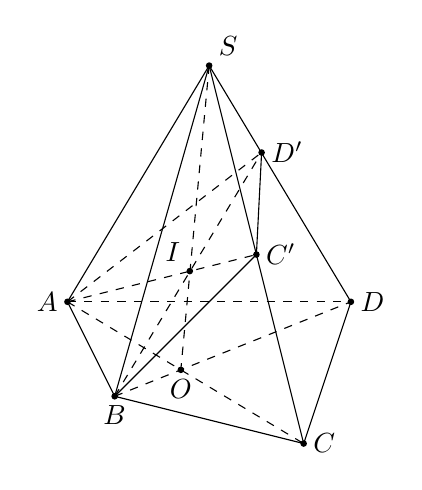
\begin{tikzpicture}[scale=.6]
				\draw (1,0)-- (2,-2)-- (6,-3)-- (7,0)--(4,5)--(1,0);
				\draw (4,5)-- (2,-2);
				\draw (4,5)-- (6,-3);
				\draw (2,-2)-- (5,1)--(5.11,3.16);
				\draw [dashed] (1,0)--(5.11,3.16);
				\draw [dashed] (1,0)-- (7,0);
				\draw [dashed] (1,0)-- (5,1);
				\draw [dashed] (1,0)-- (6,-3);
				\draw [dashed] (2,-2)-- (7,0);
				\draw [dashed] (4,5)--(3.4,-1.44);
				\draw [dashed] (2,-2)--(5.11,3.16);
				\fill (1,0) circle (.07) node [left]{$A$};
				\fill (2,-2) circle (.07) node [below]{$B$};
				\fill (6,-3) circle (.07) node [right]{$C$};
				\fill (4,5) circle (.07) node [above right]{$S$};
				\fill (7,0) circle (.07) node [right]{$D$};
				\fill (5,1) circle (.07) node [right]{$C'$};
				\fill (5.11,3.16) circle (.07) node [ right]{$D'$};
				\fill (3.4,-1.44) circle (.07) node [below]{$O$};
				\fill (3.59,0.65) circle (.07) node [above left]{$I$};
	\end{tikzpicture}}}
\end{ex}
%Câu 16
\begin{ex}%[1K4BB-3]
	Cho mặt phẳng $(\alpha)$ chứa hình bình hành $ABCD $, một điểm $S$ nằm ngoài $(\alpha)$. Gọi $d$
	là giao tuyến của hai mặt phẳng $(SAB)$ và $(SCD)$. Mệnh đề nào sau đây đúng?
	\choice
	{$d$ là đường thẳng $SK$ với $K$ là trung điểm của $AB$}
	{$d$ là đường thẳng qua điểm $S$ và song song với $AC$}
	{$d$ là đường thẳng $SO$ với $O=AC\cap BD$}
	{\True $d$ là đường thẳng qua điểm $S$ và song song với $AB$}
	\loigiai{
		\immini{
			Ta có $S$ là điểm chung của hai mặt phẳng $(SAB)$ và $(SCD)$.\\
			$\heva{&AB \parallel CD\\ &AB \subset (SAB)\\ &CD \subset (SCD)}.$\\
			Vậy giao tuyến là $d$ với $d$ là đường thẳng qua điểm $S$ và song song với $AB$.}{
		\begin{tikzpicture}[>=stealth,line join=round,line cap=round,font=\footnotesize,scale=1]
			\tikzset{
				pics/hinhChopTuGiacDeu/.style  n args={5}{
					code={
						\tikzset{
							declare function={a=4;b=2;h=3;goc=-120;}
						}	
						\path 
						(0,0)coordinate (#1)+(0:a)coordinate (#2)+(goc:b)coordinate (#4)+(80:h)coordinate (#5)
						($(#2)+(#4)-(#1)$)coordinate (#3)
						;
					}
			}}
			\path 
			(0,0)pic[scale=.8]{hinhChopTuGiacDeu={A}{B}{C}{D}{S}}
			;
			\foreach \pointo/\pointt in {S/B,S/C,S/D,B/C,C/D}{
				\draw[fill=black](\pointo)--(\pointt);
			}
			\foreach \pointo/\pointt in {S/A,A/B,A/D}{
				\draw[fill=black,dashed](\pointo)--(\pointt);
			}
			\foreach \point/\goc in {S/90,A/180,B/10,D/190,C/-20}{
				\draw[fill=black](\point)circle(.8pt)+(\goc:2mm)node[scale=.8]{$\point$};
			}
		\end{tikzpicture}
	}}
\end{ex}
%Câu 17
\begin{ex}%[1K4BA-2]
	Cho tứ diện $ABCD$. Gọi $M, N, P, Q $ lần lượt là trung điểm của các cạnh $AB, AD, CD, BC$. Mệnh đề nào sau đây {\bf {sai}}?
	\choice
	{$MNPQ$ là hình bình hành}
	{$BD \parallel PQ$ và $PQ =\dfrac{1}{2}BD$}
	{\True $MQ$ và $NP$ chéo nhau}
	{$MN \parallel BD$ và $MN =\dfrac{1}{2}BD$}
	\loigiai
	{\immini {
			\begin{itemize}
				\item Do $MN$ là đường trung bình của $\triangle ABD\break \Rightarrow MN \parallel BD$ và $MN =\dfrac{1}{2}BD$.
				\item Do $PQ$ là đường trung bình của $\triangle CBD\break \Rightarrow PQ \parallel BD$ và $PQ =\dfrac{1}{2}BD \Rightarrow$ tứ giác $MNPQ$ là hình bình hành.
				\item  Do $PQ$ là đường trung bình của $\triangle BCD\break \Rightarrow PQ \parallel BD$ và $PQ =\dfrac{1}{2}BD$.
				\item Do tứ giác $MNPQ$ là hình bình hành nên $MQ\parallel NP$.
			\end{itemize}
		}{
		\begin{tikzpicture}[>=stealth,line join=round,line cap=round,font=\footnotesize,scale=1]
			\tikzset{
				pics/chopTamGiac/.style n args={4}{
					code={
						\tikzset{declare function={a=4;b=2;h=3;goc=-60;}}
						\path 
						(0,0)coordinate (#1)+(0:a)coordinate (#3)+
						(goc:b)coordinate (#2)+(70:h)coordinate (#4)
						
						;
						\foreach \pointo/\pointt in {#4/#1,#1/#2,#2/#3,#3/#4,#4/#2}{
							\draw[fill=black](\pointo)--(\pointt);
						}
						\foreach \pointo/\pointt in {#1/#3}{
							\draw[fill=black,dashed](\pointo)--(\pointt);
						}
						
					}
			}}
			\path 
			(0,0)coordinate (a)pic[scale=1.4]{chopTamGiac={B}{D}{C}{A}}
			($(A)!.5!(B)$) coordinate (M)
			($(A)!.5!(D)$)coordinate (N)
			($(D)!.5!(C)$)coordinate (P)
			($(C)!.5!(B)$)coordinate (Q)
			;
			\foreach \pointo/\pointt in {M/N,N/P}{
				\draw[fill=black](\pointo)--(\pointt);
			}
			\foreach \pointo/\pointt in {M/Q,Q/P}{
				\draw[fill=black,dashed](\pointo)--(\pointt);
			}
			\foreach \point/\goc in {D/-90,A/135,B/190,C/-10,M/135,N/200,P/-45,Q/45}{
				\draw[fill=black](\point)circle(.8pt)+(\goc:2mm)node[scale=.8]{$\point$};
			}
	\end{tikzpicture}
}
	}
\end{ex}
%Câu 18
\begin{ex}%[1K4YB-1]
	Cho hình hộp $ABCD.A'B'C'D'$. Mệnh đề nào sau đây \textbf{sai}?
	\choice
	{$AD$ song song với $(A'B'C'D')$}
	{$DD'$ song song với $(ABB'A')$}
	{\True $B'C'$ song song với $(BDD')$}
	{$AB$ song song với $(CDD'C')$}
	\loigiai{
		\immini{Dựa vào hình vẽ ta có\\ $\heva{&B'C' \parallel BC\\ &BC \cap (BDD')=B}$ \\
			nên $B'C'$ không song song với $(BDD')$.}{
		\begin{tikzpicture}[>=stealth,line join=round,line cap=round,font=\footnotesize,scale=1]
			\tikzset{
				pics/hhChuNhat/.style n args={8}{
					code={
						\tikzset{
							declare function={a=4;b=2;goc=-120;h=3;}
						}
						\path 
						(0,0)coordinate (#1)+(0:a)coordinate (#2)+(goc:b)coordinate (#4)+(90:h)coordinate (#5)
						($(#2)+(#4)-(#1)$)coordinate (#3)
						;
						\foreach \pone/\pname in {#2/#6,#3/#7,#4/#8}{
							\path 
							($(\pone)+(#5)-(#1)$)coordinate (\pname)
							;
						}
						\foreach \pointo/\pointt in {#1/#2,#1/#4,#1/#5}{
							\draw[fill=black,dashed](\pointo)--(\pointt);
						}
						\foreach \pointo/\pointt in {#2/#3,#3/#4,#5/#6,#6/#7,#7/#8,#8/#5,#2/#6,#3/#7,#4/#8}{
							\draw[fill=black](\pointo)--(\pointt);
						}
					}
				}
			}
			\path 
			(0,0) pic[scale=.8]{hhChuNhat={A'}{B'}{C'}{D'}{A}{B}{C}{D}}
			;
			\foreach \pointo/\pointt in {D/B}{
				\draw[fill=black](\pointo)--(\pointt);
			}
			\foreach \pointo/\pointt in {D'/B}{
				\draw[fill=black,dashed](\pointo)--(\pointt);
			}
			\foreach \point/\goc in {A/90,B/90,D/190,C/-10,A'/135,B'/-10,C'/-80,D'/190}{
				\draw[fill=black](\point)circle(.8pt)+(\goc:2mm)node[scale=.8]{$\point$};
			}
		\end{tikzpicture}
		}
	}
\end{ex}
%Câu 19
\begin{ex}%[1K4YB-1]
	Cho đường thẳng $a$, $d$ và mặt phẳng $(\alpha)$, $(\beta)$ thỏa mãn $\heva{&a\parallel (\alpha)\\&a\subset (\beta)\\&d=(\alpha)\cap (\beta)}$. Khẳng định nào sau đây đúng?
	\choice
	{$a$ trùng $d$}
	{\True $a\parallel d$}
	{$a$ cắt $d$}
	{$a$ và $d$ chéo nhau}
	\loigiai
	{Ta có $\heva{&a\parallel (\alpha)\\&a\subset (\beta)\\&d=(\alpha)\cap (\beta)}\Rightarrow a\parallel d$.
	}
\end{ex}
%Câu 20
\begin{ex}%[1K4BC-1]
	Hình lăng trụ có các mặt bên là hình gì?
	\choice
	{Hình thoi}
	{Hình chữ nhật}
	{\True Hình bình hành}
	{Hình vuông}
	\loigiai{
		Hình lăng trụ có các mặt bên là các hình bình hành.
	}
\end{ex}
%Câu 21
\begin{ex}%[1K4BB-2]
	Cho hình chóp $S.ABCD$ có đáy $ABCD$ là hình bình hành. Gọi $I,J$ lần lượt là trọng tâm của $\triangle SAB,\triangle SAD$ và $E,F$ là trung điểm của $AB,AD$. Mệnh đề nào dưới đây đúng?
	\choice
	{\True $IJ\parallel (SBD)$}
	{$IJ\parallel (SAD)$}
	{$IJ\parallel (SAB)$}
	{$IJ\parallel (SFE)$}
	\loigiai{
		\immini{
			Xét $\triangle SFE$ có:
			$\dfrac{SJ}{SF}=\dfrac{SI}{SE}=\dfrac{2}{3}$ (do $I,J$ là trọng tâm của $\triangle SAB,\triangle SAD$).
			Áp dụng định lý Thales đảo vào $\triangle SEF$ ta có $IJ\parallel EF$. $(1)$\\
			Mà $EF \parallel BD\subset (SBD)$. $(2)$\\ 
			Từ $(1)$ và $(2)$ suy ra $IJ\parallel (SBD)$.
		}{
			\begin{tikzpicture}[>=stealth,line join=round,line cap=round,font=\footnotesize,scale=1]
				\tikzset{
					pics/hinhChopTuGiacDeu/.style  n args={5}{
						code={
							\tikzset{
								declare function={a=4;b=2;h=3;goc=-120;}
							}	
							\path 
							(0,0)coordinate (#1)+(0:a)coordinate (#2)+(goc:b)coordinate (#4)+(80:h)coordinate (#5)
							($(#2)+(#4)-(#1)$)coordinate (#3)
							;
						}
				}}	
				\path 
				(0,0)pic {hinhChopTuGiacDeu={C}{B}{A}{D}{S}}
				($(B)!.5!(A)$)coordinate (E) ($(A)!.5!(D)$)coordinate (F)
				($(S)!2/3!(F)$)coordinate (J) ($(S)!2/3!(E)$)coordinate (I)
				(intersection of B--I and D--J)coordinate (M)
				;
				\foreach \pointo/\pointt in {S/A,S/B,A/B,A/D,S/E,S/F,D/M,B/M,S/D}{
					\draw[fill=black](\pointo)--(\pointt);
				}
				\foreach \pointo/\pointt in {S/C,C/D,C/B,I/J,B/D,E/F}{
					\draw[fill=black,dashed](\pointo)--(\pointt);
				}
				\foreach \point/\goc in {S/90,C/135,B/-10,D/190,A/-80,E/-60,F/-90,I/45,J/180}{
					\draw[fill=black](\point)circle(.8pt)+(\goc:2mm)node[scale=.8]{$\point$};
				}
			\end{tikzpicture}
		}
	}
\end{ex}
%Câu 22
\begin{ex}%[1K4BA-3]
	Cho hình chóp $S.ABCD$ có đáy $ABCD$ là hình thang, $AD\parallel BC$, $AD=2BC$. Gọi $M$ là trung điểm $SA$. Mặt phẳng $(MBC)$ cắt hình chóp $S.ABCD$ theo thiết diện là
	\choice
	{một hình tứ giác (không là hình thang)}
	{một hình thang (không là hình bình hành)}
	{\True một hình bình hành}
	{một tam giác}
	\loigiai{
		\immini{Gọi $N$ là giao của $SD$ và mặt phẳng $(MBC)$.\\
		Do các mặt phẳng $(MBC)$ và $(SAD)$ lần lượt chứa hai đường song song là $BC$ và $AD$, nên giao tuyến của chúng cũng song song với hai đường đó, tức $MN\parallel AD$.\\
		Suy ra $N$ là trung điểm của $SD$.\\
		Khi đó, $MN$ là đường trung bình của tam giác $SAD$, suy ra $MN=\dfrac12 AD=BC$.\\
		Vậy, thiết diện $BCNM$ là một hình bình hành.
		}{
		\begin{tikzpicture}[>=stealth,line join=round,line cap=round,font=\footnotesize,scale=1]
			\tikzset{
				pics/hinhChopTuGiacHinhThang/.style  n args={5}{
					code={
						\tikzset{
							declare function={a=3.5;b=1.5;h=2.5;goc=-145;}
						}	
						\path 
						(0,0)coordinate (#1)+(0:a)coordinate (#2)+(goc:b)coordinate (#4)+(80:h)coordinate (#5)
						($(#2)+(#4)-(#1)$)coordinate (c)
						($(c)!.5!(#4)$)coordinate (#3)
						;
					}
			}}	
			\path 
			(0,0)pic {hinhChopTuGiacHinhThang={A}{D}{C}{B}{S}}
			($(A)!.5!(S)$)coordinate (M) ($(D)!.5!(S)$)coordinate (N)
			;
			\foreach \pointo/\pointt in {S/B,S/C,S/D,B/C,C/D,N/C}{
				\draw[fill=black](\pointo)--(\pointt);
			}
			\foreach \pointo/\pointt in {A/B,A/D,M/N,M/B,S/A}{
				\draw[fill=black,dashed](\pointo)--(\pointt);
			}
			\foreach \point/\goc in {S/90,M/135,A/145,B/190,C/-80,D/-10,N/45}{
				\draw[fill=black](\point)circle(.8pt)+(\goc:2mm)node[scale=.8]{$\point$};
			}
		\end{tikzpicture}
		
	}
}
\end{ex}
%Câu 23
\begin{ex}%[1K4BB-2]
	Cho hình chóp $S.ABCD$ có đáy $ABCD$ là hình bình hành. Gọi $M$, $N$ lần lượt là trung điểm của $SA$, $SB$.
	Mệnh đề nào sau đây là mệnh đề đúng?
	\choice
	{\True $MN \parallel (ACD)$}
	{$MN \parallel (SAC)$}
	{$MN \parallel (SAB)$}
	{$MN \parallel (SBD)$}
	\loigiai{
		\immini
		{ Vì $M$, $N$ lần lượt là trung điểm của $SA$, $SB$ nên $MN$ là đường trung bình trong tam giác $SAB$, suy ra $MN \parallel AB$.\\ Mà $AB \subset (ACD)$ nên $MN \parallel (ACD)$.
		}
		{
\begin{tikzpicture}[>=stealth,line join=round,line cap=round,font=\footnotesize,scale=1]
	\tikzset{
		pics/hinhChopTuGiacDeu/.style  n args={5}{
			code={
				\tikzset{
					declare function={a=3.5;b=2;h=2.5;goc=-120;}
				}	
				\path 
				(0,0)coordinate (#1)+(0:a)coordinate (#2)+(goc:b)coordinate (#4)+(80:h)coordinate (#5)
				($(#2)+(#4)-(#1)$)coordinate (#3)
				;
			}
	}}
	\path 
	(0,0)pic[scale=.8] {hinhChopTuGiacDeu={D}{C}{B}{A}{S}}
	($(A)!.5!(S)$)coordinate (M) ($(B)!.5!(S)$)coordinate (N)
	;	
	\foreach \pointo/\pointt in {S/A,S/B,S/C,M/N,A/B,B/C}{
		\draw[fill=black](\pointo)--(\pointt);
	}
	\foreach \pointo/\pointt in {S/D,D/A,D/C}{
		\draw[fill=black,dashed](\pointo)--(\pointt);
	}
	\foreach \point/\goc in {S/90,A/190,D/135,B/-60,C/-10,M/135,N/45}{
		\draw[fill=black](\point)circle(.8pt)+(\goc:2mm)node[scale=.8]{$\point$};
	}
\end{tikzpicture}
		}
	}
\end{ex}
%Câu 24
\begin{ex}%[1K4BA-2]
	Cho tứ diện $ABCD$. Gọi $G$ và $E$ lần lượt là trọng tâm của tam giác $ABD$ và $ABC$. Mệnh đề nào dưới đây đúng?
	\choice
	{\True $GE\parallel CD$}
	{GE cắt AD}
	{ GE cắt BC}
	{GE và CD chéo nhau}
	\loigiai{
		\immini{
			Gọi $M,N$ lần lượt là trung điểm của $BC, BD$.\\
			Vì $G$ và $E$ lần lượt là trọng tâm của tam giác $ABD$ và $ABC$ nên $GE\parallel MN$.\\
			Vậy $GE\parallel CD$.
		}{
	\begin{tikzpicture}[>=stealth,line join=round,line cap=round,font=\footnotesize,scale=1]
		\tikzset{
			pics/chopTamGiac/.style n args={4}{
				code={
					\tikzset{declare function={a=4;b=2;h=3;goc=-60;}}
					\path 
					(0,0)coordinate (#1)+(0:a)coordinate (#3)+
					(goc:b)coordinate (#2)+(70:h)coordinate (#4)
					
					;
					\foreach \pointo/\pointt in {#4/#1,#1/#2,#2/#3,#3/#4,#4/#2}{
						\draw[fill=black](\pointo)--(\pointt);
					}
					\foreach \pointo/\pointt in {#1/#3}{
						\draw[fill=black,dashed](\pointo)--(\pointt);
					}
					
				}
		}}
		\path 
		(0,0)coordinate (a)pic[scale=.8]{chopTamGiac={B}{C}{D}{A}}
		($(B)!.5!(C)$)coordinate (M)($(B)!.5!(D)$)coordinate (N)
		($(A)!2/3!(M)$)coordinate (E)($(A)!2/3!(N)$)coordinate (G)
		;
		\foreach \pointo/\pointt in {A/M}{
			\draw[fill=black](\pointo)--(\pointt);
		}
		\foreach \pointo/\pointt in {A/N,E/G,M/N}{
			\draw[fill=black,dashed](\pointo)--(\pointt);
		}
		\foreach \point/\goc in {D/-10,A/135,B/190,C/-90,M/-135,N/45,E/135,G/60}{
			\draw[fill=black](\point)circle(.8pt)+(\goc:2mm)node[scale=.8]{$\point$};
		}
	\end{tikzpicture}
	}}
\end{ex}
%Câu 25
\begin{ex}%[1K4BA-3]
	Cho hình chóp $S.ABCD$ có đáy $ABCD$ là hình bình hành. Giao tuyến của hai mặt phẳng $(SAB)$ và $(SCD)$ là
	\choice
	{Đường thẳng đi qua $S$ và song song với đường thẳng $BD$}
	{\True Đường thẳng đi qua $S$ và song song với đường thẳng $CD$}
	{Đường thẳng đi qua $S$ và song song với đường thẳng $AC$}
	{Đường thẳng đi qua $S$ và song song với đường thẳng $AD$}
	\loigiai{
		\immini{Ta có $\heva{&S\in (SAB)\cap (SCD)\\&AB\parallel CD\\&AB\subset (SAB), CD\subset (SCD)}$\\
			$\Rightarrow (SAB)\cap (SCD)=d$, $d$ qua $S$ và $d\parallel CD$.
		}
		{
\begin{tikzpicture}[>=stealth,line join=round,line cap=round,font=\footnotesize,scale=1]
	\tikzset{
		pics/hinhChopTuGiacDeu/.style  n args={5}{
			code={
				\tikzset{
					declare function={a=4;b=2;h=3;goc=-120;}
				}	
				\path 
				(0,0)coordinate (#1)+(0:a)coordinate (#2)+(goc:b)coordinate (#4)+(80:h)coordinate (#5)
				($(#2)+(#4)-(#1)$)coordinate (#3)
				;
			}
	}}
	\path 
	(0,0)pic[scale=.8] {hinhChopTuGiacDeu={A}{B}{C}{D}{S}}
	($(S)+(B)-(A)$)coordinate (d)node[above]{$d$}
	;
	\draw[shorten <=-.5cm,shorten >=-.5cm] (S)--(d);
	\foreach \pointo/\pointt in {S/B,S/D,S/C,B/C,C/D}{
		\draw[fill=black](\pointo)--(\pointt);
	}
	\foreach \pointo/\pointt in {S/A,A/B,A/D}{
		\draw[fill=black,dashed](\pointo)--(\pointt);
	}
	\foreach \point/\goc in {S/90,A/135,D/190,C/-80,B/-10}{
		\draw[fill=black](\point)circle(.8pt)+(\goc:2mm)node[scale=.8]{$\point$};
	}	
\end{tikzpicture}
		}
	}
\end{ex}
%Câu 26
\begin{ex}%[1K4BB-2]
	Cho hình chóp $S.ABCD$ có đáy $ABCD$ là hình bình hành. Gọi $M,N$ lần lượt là trung điểm các cạnh $DC,BC,SA$. Gọi $H$ là giao điểm của $AC$ và $MN$. Trong các khẳng định sau, khẳng định nào \textbf{sai}?
	\choice
	{\True $MN \parallel (ABCD)$}
	{$MN$ giao mặt $(SAC)$ tại $H$}
	{$MN \parallel (SBD)$}
	{$MN$ chéo $SC$}
	\loigiai{
		\immini{
			\begin{itemize}\vspace*{-24pt}
				\item Vì $MN \subset (ABCD)$ và $SC$ cắt $(ABCD)$ tại $C \notin MN$ nên $MN$ và $SC$ chéo nhau.
				\item $\heva{&MN \parallel BD\\&BD \subset (SBD)} \,\Rightarrow\, MN \parallel (SBD)$.
				\item $MN \subset (ABCD)$.
				\item $\heva{&MN \cap AC=H\\&AC \subset (SAC)} \,\Rightarrow\, MN \cap (SAC)=H$.
			\end{itemize}
		}{
			\begin{tikzpicture}[>=stealth,line join=round,line cap=round,font=\footnotesize,scale=1]
				\tikzset{
					pics/hinhChopTuGiacDeu/.style  n args={5}{
						code={
							\tikzset{
								declare function={a=4;b=2;h=3;goc=-120;}
							}	
							\path 
							(0,0)coordinate (#1)+(0:a)coordinate (#2)+(goc:b)coordinate (#4)+(80:h)coordinate (#5)
							($(#2)+(#4)-(#1)$)coordinate (#3)
							;
						}
				}}
				\path 
				(0,0)pic[scale=.8] {hinhChopTuGiacDeu={A}{D}{C}{B}{S}}
				($(B)!.5!(C)$)coordinate (N)($(D)!.5!(C)$)coordinate (M)
				(intersection of M--N and A--C)coordinate (H)
				;
				
				\foreach \pointo/\pointt in {S/B,S/D,S/C,B/C,C/D}{
					\draw[fill=black](\pointo)--(\pointt);
				}
				\foreach \pointo/\pointt in {S/A,A/B,A/D,A/C,M/N,B/D}{
					\draw[fill=black,dashed](\pointo)--(\pointt);
				}
				\foreach \point/\goc in {S/90,A/135,B/190,C/-80,D/-10,H/90,M/-30,N/-90}{
					\draw[fill=black](\point)circle(.8pt)+(\goc:2mm)node[scale=.8]{$\point$};
				}	
			\end{tikzpicture}
		}
	}
\end{ex}
%Câu 27
\begin{ex}%[1K4BB-2]
	Cho hình chóp $S.ABCD$ có đáy $ABCD$ là hình bình hành. Chọn khẳng định đúng.
	\choice
	{$CD\parallel (SAC)$}
	{\True $CD\parallel (SAB)$}
	{$BD\parallel (SAD)$}
	{$BD\parallel (SAC)$}
	\loigiai{
		\immini{
			Ta thấy $BD$ và $CD$ cắt $(SAC)$.\\
			Do $CD\parallel AB$, mà $AB\subset (SAB)$ và $CD\not\subset (SAB)$ nên suy ra $CD\parallel (SAB)$.
		}{
			\begin{tikzpicture}[>=stealth,line join=round,line cap=round,font=\footnotesize,scale=1]
				\tikzset{
					pics/hinhChopTuGiacDeu/.style  n args={5}{
						code={
							\tikzset{
								declare function={a=4;b=2;h=3;goc=-120;}
							}	
							\path 
							(0,0)coordinate (#1)+(0:a)coordinate (#2)+(goc:b)coordinate (#4)+(80:h)coordinate (#5)
							($(#2)+(#4)-(#1)$)coordinate (#3)
							;
						}
				}}
				\path 
				(0,0)pic[scale=.8] {hinhChopTuGiacDeu={A}{D}{C}{B}{S}}
				;
				
				\foreach \pointo/\pointt in {S/B,S/D,S/C,B/C,C/D}{
					\draw[fill=black](\pointo)--(\pointt);
				}
				\foreach \pointo/\pointt in {S/A,A/B,A/D,A/C,B/D}{
					\draw[fill=black,dashed](\pointo)--(\pointt);
				}
				\foreach \point/\goc in {S/90,A/135,B/190,C/-80,D/-10}{
					\draw[fill=black](\point)circle(.8pt)+(\goc:2mm)node[scale=.8]{$\point$};
				}	
			\end{tikzpicture}
		}
		
	}
\end{ex}
%Câu 28
\begin{ex}%[1K4BB-5]
	Cho tứ diện $ABCD$. Gọi $M$ là trung điểm của cạnh $AB$. Cắt tứ diện $ABCD$ bởi mặt phẳng qua $M$ và song song với hai cạnh $BC$; $AD$. Thiết diện thu được là hình gì?
	\choice
	{\True Hình bình hành}
	{Ngũ giác}
	{Tam giác vuông}
	{Tam giác đều}
	\loigiai{
		\immini{Gọi $N$, $P$, $Q$ lần lượt là trung điểm các cạnh $AC$, $CD$, $BD$.\\
			Khi đó $MN$ và $PQ$ cùng song song với $BC$ và cùng bằng nửa $BC$.\\
			Suy ra $MNPQ$ là hình bình hành (đương nhiên lúc đó $M$, $N$, $P$, $Q$ đồng phẳng)\\
			Ngoài ra $NP$ song song với $AD$ nên $(MNPQ)$ là thiết diện qua $M$ và song song với cả $BC$ lẫn $AD$.}
		{\begin{tikzpicture}[line width=0.6pt,line cap=round,line join=round,>=stealth,scale=1]
				\coordinate[label=left:{$A$}] (A) at (0,0);
				\coordinate[label=below:{$C$}] (C) at (1.3,-1.5);
				\coordinate[label=right:{$D$}] (D) at (4,0);
				\coordinate[label={$B$}] (B) at (1.7,2.3);
				\coordinate[label=left:{$M$}] (M) at ($(A)!0.5!(B)$);
				\coordinate[label=below:{$N$}] (N) at ($(A)!0.5!(C)$);
				\coordinate[label=below:{$P$}] (P) at ($(C)!0.5!(D)$);
				\coordinate[label=right:{$Q$}] (Q) at ($(B)!0.5!(D)$);
				\draw (B)--(A)--(C)--(B)--(D)--(C) (M)--(N) (P)--(Q);
				\draw[dashed] (A)--(D) (N)--(P) (M)--(Q);
	\end{tikzpicture}}}
\end{ex}
%Câu 29
\begin{ex}%[1K4BC-2]
	Cho hình chóp $S.ABCD$, có đáy $ABCD$ là hình bình hành tâm $O$. Gọi $M,N$ lần lượt là trung điểm $SA,SD$. Mặt phẳng $\left(OMN\right)$ song song với mặt phẳng nào sau đây?
	\choice
	{$\left(ABCD\right)$}
	{\True $\left(SBC\right)$}
	{$\left(SAB\right)$}
	{$\left(SCD\right)$}
	\loigiai{
		\immini{
			Vì $ABCD$ là hình bình hành nên $O$ là trung điểm $AC,BD$.\\
			Do đó $MO \parallel SC\Rightarrow MO\parallel \left(SBC\right)$\\
			Và $NO \parallel SB \Rightarrow NO\parallel \left(SBC\right)$\\
			Suy ra $\left(OMN\right)\parallel \left(SBC\right)$.}{
		\begin{tikzpicture}[>=stealth,line join=round,line cap=round,font=\footnotesize,scale=1]
			\tikzset{
				pics/hinhChopTuGiacDeu/.style  n args={5}{
					code={
						\tikzset{
							declare function={a=4;b=2;h=3;goc=-135;}
						}	
						\path 
						(0,0)coordinate (#1)+(0:a)coordinate (#2)+(goc:b)coordinate (#4)+(80:h)coordinate (#5)
						($(#2)+(#4)-(#1)$)coordinate (#3)
						;
					}
			}}
			\path 
			(0,0)pic[scale=.8] {hinhChopTuGiacDeu={A}{D}{C}{B}{S}}
			(intersection of A--C and B--D)coordinate (O)
			($(A)!.5!(S)$)coordinate (M) ($(D)!.5!(S)$)coordinate (N)
			;
			
			\foreach \pointo/\pointt in {S/B,S/D,S/C,B/C,C/D}{
				\draw[fill=black](\pointo)--(\pointt);
			}
			\foreach \pointo/\pointt in {S/A,A/B,A/D,A/C,B/D,M/N,N/O,M/O}{
				\draw[fill=black,dashed](\pointo)--(\pointt);
			}
			\foreach \point/\goc in {S/90,A/135,B/190,C/-80,D/-10,O/-90,M/180,N/45}{
				\draw[fill=black](\point)circle(.8pt)+(\goc:2mm)node[scale=.8]{$\point$};
			}	
		\end{tikzpicture}
	}}
\end{ex}
%Câu 30
\begin{ex}%[1K4Y0-1]
	Trong không gian, nhận xét nào sau đây là đúng?
	\choice
	{Hình biểu diễn của một góc phải là một góc bằng nó}
	{Qua ba điểm xác định duy nhất một mặt phẳng}
	{\True Qua ba điểm phân biệt không thẳng hàng xác định duy nhất một mặt phẳng}
	{Qua ba điểm phân biệt xác định duy nhất một mặt phẳng}
	\loigiai{
		Theo điều kiện xác định mặt phẳng trong không gian.
	}
\end{ex}
%Câu 31
\begin{ex}%[1K4KB-5]
	Cho hình chóp $S.ABCD$, $G$ là điểm nằm trong tam giác $SCD$, $E$, $F$ lần lượt là trung điểm của $AB$ và $AD$. Thiết diện của hình chóp khi cắt bỏi mặt phẳng $(EFG)$ là
	\choice
	{\True ngũ giác}
	{tam giác}
	{lục giác}
	{tứ giác}
	\loigiai{
		\immini{
			Gọi $H$ là giao điểm của $SG$ và $CD$, $I$ là giao điểm của $FH$ và $BD$. Nối $SI$ cắt $FG$ tại $J$. Khi đó, ta có $J\in (EFG)\cap (SBD)$. Gọi $K$, $L$ lần lượt là giao điểm của $(EFG)$ với $SB$, $SD$. Do $EF\parallel BD$ nên giao tuyến $KL$ của hai mặt phẳng $(EFG)$, $(SBD)$ đi qua $J$ và song song với $BD$. Gọi $M$ là giao điểm của $LG$ và $SC$, khi đó ngũ giác $EFLMK$ là thiết diện của hình chóp $S.ABCD$ cắt bởi mặt phẳng $(EFG)$.
		}
		{
		\begin{tikzpicture}[>=stealth,line join=round,line cap=round,font=\footnotesize,scale=1]
			\tikzset{
				pics/hinhChopTuGiacthuong/.style  n args={5}{
					code={
						\tikzset{
							declare function={a=4;b=1.2;h=3;goc=-70;goc2=-45;c=3;}
						}	
						\path 
						(0,0)coordinate (#1)+(0:a)coordinate (#2)+(goc:b)coordinate (#4)+(80:h)coordinate (#5)+(goc2:c)coordinate (#3)		
						;
					}
			}}
			\path 
			(0,0)pic {hinhChopTuGiacthuong={C}{D}{A}{B}{S}}
			($(C)!.4!(D)$)coordinate (H)($(H)!.3!(S)$)coordinate (G)
			($(A)!.5!(B)$)coordinate (E)($(A)!.5!(D)$)coordinate (F)
			(intersection of H--F and B--D)coordinate (I)
			(intersection of S--I and F--G)coordinate (J)
			($(B)+(J)-(I)$)coordinate (d)
			(intersection of S--B and J--d)coordinate (K)
			(intersection of S--D and J--d)coordinate (L)
			(intersection of S--C and L--G)coordinate (M)
			;
			\fill[pattern=north east lines,opacity=.2] 
			(M)--(K)--(E)--(F)--(L)--cycle
			;
			\foreach \pointo/\pointt in {S/C,S/B,S/A,S/D,B/C,B/A,A/D,M/K,K/E,L/F}{
				\draw[fill=black](\pointo)--(\pointt);
			}
			\foreach \pointo/\pointt in {C/D,M/L,K/L,G/F,H/F,B/D,E/F,S/H,S/I}{
				\draw[fill=black,dashed](\pointo)--(\pointt);
			}
			\foreach \point/\goc in {S/90,C/190,B/190,K/180,E/-150,A/-90,F/-45,D/-10,L/45,H/60,G/60,I/-100,J/80,M/135}{
				\draw[fill=black](\point)circle(.8pt)+(\goc:1.6mm)node[scale=.7]{$\point$};
			}
		\end{tikzpicture}
		}
	}
\end{ex}
%Câu 32
\begin{ex}%[1K4YC-1]
	Trong không gian, cho các đường thẳng $a,b$ và mặt phẳng $(P)$, $(Q)$. Tìm mệnh đề đúng trong các mệnh đề sau?
	\choice
	{Nếu $(P)\parallel (Q)$ và $a\subset(P)$, $b\subset (Q)$ thì $a\parallel b$}
	{\True Nếu $(P)\parallel (Q)$ và $a\subset(P)$ thì $a\parallel (Q)$}
	{Nếu $a\parallel b$ và $a\subset(P)$, $b\subset (Q)$ thì $(P)\parallel (Q)$}
	{Nếu $a\parallel (P)$ và $b\parallel (Q)$ thì $a\parallel b$}
	\loigiai{
		Cho hai mặt phẳng song song nếu đường thẳng nào nằm trong mặt phẳng này thì song song với mặt phẳng còn lại.}
\end{ex}
%Câu 33
\begin{ex}%[1H2B3-1]
	Cho hai đường thẳng phân biệt $a$, $b$ và mặt phẳng $(\alpha)$. Giả sử $a \parallel (\alpha)$ và $b \parallel (\alpha)$. Mệnh đề nào sau đây \textbf{đúng}?
	\choice
	{$a$ và $b$ chéo nhau}
	{\True $a$ và $b$ hoặc song song hoặc chéo nhau hoặc cắt nhau}
	{$a$ và $b$ hoặc song song hoặc chéo nhau}
	{$a$ và $b$ không có điểm chung}
	\loigiai
	{
		Cho hai đường thẳng phân biệt $a$, $b$ và mặt phẳng $(\alpha)$. Giả sử $a\parallel (\alpha)$ và $b\parallel (\alpha)$. Khi đó, hai đường thẳng $a$ và $b$ hoặc song song hoặc chéo nhau hoặc cắt nhau.
	}
\end{ex}
%Câu 34
\begin{ex}%[1K4YD-1]
	Khẳng định nào sau đây \textbf{sai}?
	\choice
	{\True Phép chiếu song song có thể biến một đường tròn thành một điểm}
	{Phép chiếu song song có thể biến một đường tròn thành một đường tròn}
	{Phép chiếu song song có thể biến một đường tròn thành một đoạn thẳng}
	{Phép chiếu song song có thể biến một đường tròn thành một elip}
	\loigiai{
		Theo tính chất của phép chiếu song song ta có phương án ``\textit{Phép chiếu song song có thể biến một đường tròn thành một điểm}'' là phương án sai.
	}
\end{ex}
%Câu 35
\begin{ex}%[1K4BB-3]
	Cho hình chóp $S.ABCD$ có đáy $ABCD$ là hình bình hành. Tìm giao tuyến của hai mặt phẳng $(SAD)$ và $(SBC)$.
	\choice
	{Đường thẳng qua điểm $S$ và song song với $AB$, $CD$}
	{$SO$ với $O$ là giao điểm của $AC$ và $BD$}
	{$SA$}
	{\True Đường thẳng qua điểm $S$ và song song với $AD$, $BC$}
	\loigiai{
		\immini{
			Ta có $\heva{&S \in (SAD) \cap (SBC)\\&AD \subset (SAD),BC \subset (SBC)\\&AD \parallel BC}$ nên giao tuyến của hai mặt phẳng $(SAD)$ và $(SBC)$ là đường thẳng $\Delta$ đi qua điểm $S$ và song song với $AD$, $BC$.
		}{
		\begin{tikzpicture}[>=stealth,line join=round,line cap=round,font=\footnotesize,scale=1]
			\tikzset{
				pics/hinhChopTuGiacDeu/.style  n args={5}{
					code={
						\tikzset{
							declare function={a=4;b=2;h=3;goc=-120;}
						}	
						\path 
						(0,0)coordinate (#1)+(0:a)coordinate (#2)+(goc:b)coordinate (#4)+(80:h)coordinate (#5)
						($(#2)+(#4)-(#1)$)coordinate (#3)
						;
					}
			}}
			\path 
			(0,0)pic[scale=.8] {hinhChopTuGiacDeu={A}{B}{C}{D}{S}}
			($(S)+(B)-(A)$)coordinate (d)node[above]{$\Delta$}
			;
			\draw[shorten <=-.5cm,shorten >=-.5cm] (S)--(d);
			\foreach \pointo/\pointt in {S/B,S/D,S/C,B/C,C/D}{
				\draw[fill=black](\pointo)--(\pointt);
			}
			\foreach \pointo/\pointt in {S/A,A/B,A/D}{
				\draw[fill=black,dashed](\pointo)--(\pointt);
			}
			\foreach \point/\goc in {S/90,A/135,D/190,C/-80,B/-10}{
				\draw[fill=black](\point)circle(.8pt)+(\goc:2mm)node[scale=.8]{$\point$};
			}	
		\end{tikzpicture}
		}
	}
\end{ex}
%Câu 36
\begin{ex}%[1K4Y0-1]
	Chọn mệnh đề {\bf sai}
	\choice
	{Có một và chỉ một đường thẳng đi qua hai điểm phân biệt}
	{Tồn tại bốn điểm không cùng thuộc một mặt phẳng}
	{\True Có vô số mặt phẳng đi qua ba điểm không thẳng hàng}
	{Nếu hai mặt phẳng phân biệt có một điểm chung thì chúng còn có một điểm chung khác nữa}
	\loigiai{
		Mệnh đề sai là \lq\lq  Có vô số mặt phẳng đi qua ba điểm không thẳng hàng\rq\rq.
	}
\end{ex}
%Câu 37
\begin{ex}%[1K4B0-1]
	Tìm mệnh đề \textbf{sai} trong các mệnh đề sau.
	\choice
	{Nếu hai mặt phẳng có một điểm chung thì chúng còn vô số điểm chung khác nữa}
	{Có một và chỉ một mặt phẳng đi qua ba điểm không thẳng hàng}
	{\True Nếu một đường thẳng có một điểm thuộc mặt phẳng thì mọi điểm của đường thẳng đều thuộc mặt phẳng đó}
	{Có một và chỉ một đường thẳng đi qua hai điểm phân biệt}
	\loigiai{
		Nếu đường thẳng $d$ có một điểm thuộc mặt phẳng $(P)$ thì $d$ cắt $(P)$ hoặc $d\subset (P)$.
	}
\end{ex}
%Câu 38
\begin{ex}%[1K4BB-3]
	Cho hình chóp $ S.ABCD $ có đáy $ ABCD $ là hình bình hành. Giao tuyến của hai mặt phẳng $ (SAD) $ và $ (SBC) $ là đường thẳng song song với đường thẳng nào sau đây?
	\choice
	{$ AC $}
	{$ BD $}
	{$ SC $}
	{\True $ AD $}
	\loigiai{
		Ta có $ \heva{&S\in(SAD)\cap(SBC)\\&AD\parallel BC\\&AD\subset(SAD)\\&BC\subset(SBC)} $ suy ra $ (SAD)\cap(SBC) =Sx$ với $ Sx\parallel AD $.
	}
\end{ex}
%Câu 39
\begin{ex}%[1K4BA-3]
	Cho hình chóp $S.ABCD$ có đáy $ABCD$ là hình thang, đáy lớn là $CD$. Gọi $M$ là trung điểm của cạnh $SA$, $N$ là giao điểm của cạnh $SB$  và mặt phẳng $(MCD)$. Mệnh đề nào sau đây là mệnh đề đúng?
	\choice
	{\True $MN \parallel CD$}
	{$MN$ và $SC$ cắt nhau}
	{$MN$ và $CD$ chéo nhau}
	{$MN$ và $SD$ cắt nhau}
	\loigiai{
		\immini{Hai mặt phẳng $(SAB)$ và $(MCD)$ lần lượt chứa hai đường thẳng song song $AB$, $CD$ và $MN$ là giao tuyến của chúng nên $MN\parallel CD.$}
		{
		\begin{tikzpicture}[>=stealth,line join=round,line cap=round,font=\footnotesize,scale=1]
				\tikzset{
					pics/hinhChopTuGiacHinhThang/.style  n args={5}{
						code={
							\tikzset{
								declare function={a=4;b=2;h=3;goc=-60;}
							}	
							\path 
							(0,0)coordinate (#1)+(0:a)coordinate (#2)+(goc:b)coordinate (#4)+(80:h)coordinate (#5)
							($(#2)+(#4)-(#1)$)coordinate (c)
							($(c)!.3!(#4)$)coordinate (#3)
							;
						}
				}}
				\path 
				(0,0)pic {hinhChopTuGiacHinhThang={D}{C}{B}{A}{S}}
				($(A)!.5!(S)$)coordinate (M)($(B)!.5!(S)$)coordinate (N)
				;	
				\foreach \pointo/\pointt in {S/A,S/B,S/D,S/C,D/M,M/N,A/B,A/D,B/C,N/C}{
					\draw[fill=black](\pointo)--(\pointt);
				}
				\foreach \pointo/\pointt in {D/C,M/C}{
					\draw[fill=black,dashed](\pointo)--(\pointt);
				}
				\foreach \point/\goc in {S/90,D/190,A/200,C/-10,B/-30,M/150,N/60}{
					\draw[fill=black](\point)circle(.8pt)+(\goc:2mm)node[scale=.8]{$\point$};
				}
		\end{tikzpicture}
	}
	}
\end{ex}
%Câu 40
\begin{ex}%[1K4YA-1]
	Cho hai đường thẳng phân biệt cùng nằm trong một mặt phẳng. Có bao nhiêu vị trí tương đối giữa hai đường thẳng đó?
	\choice
	{\True $2$}
	{$4$}
	{$1$}
	{$3$}
	\loigiai{
		Hai đường thẳng đồng phẳng có $2$ vị trí tương đối, đó là cắt nhau và song song.
	}
\end{ex}
%Câu 41
\begin{ex}%[1K4BB-5]
	Cho tứ diện $ABCD$ và điểm $M$  ở trên cạnh $BC$ (khác $B$ và $C$). Mặt phẳng $\left( \alpha  \right)$ qua $M$ song song với $AB$ và $CD$. Thiết diện của $\left( \alpha  \right)$ với tứ diện là
	\choice
	{Hình chữ nhật}
	{Hình thang}
	{\True Hình bình hành}
	{Hình thoi}
	\loigiai{
		\immini{Ta có $\heva{(&\alpha)\parallel AB\\
				&M\in	(\alpha)\cap (ABC)} \Rightarrow (\alpha)\cap (ABC)=MN\parallel AB$ với $N\in AC$.\\
			$\heva{(&\alpha)\parallel CD\\
				&M\in	(\alpha)\cap (DBC)} \Rightarrow (\alpha)\cap (DBC)=MP\parallel CD$ với $P\in AC$.\\
			$\heva{(&\alpha)\parallel AB\\
				&P\in	(\alpha)\cap (ABD)} \Rightarrow (\alpha)\cap (ABD)=PQ\parallel AB$ với $\in AC$.\\
			Khi đó $(\alpha)\cap (ACD)=QN.$ Mà $(\alpha)\parallel CD$ nên $QN\parallel CD$.\\
			Do đó $MN\parallel PQ, QN\parallel MP$ hay $MNPQ$ là hình bình hành.\\
			Ta có $\widehat{(AB,CD)}=\widehat{(MN,MP)}$ nên $MNPQ$ không thể là hình chữ nhật.\\
			Vì $M$ bất kỳ trên $BC$ nên $MN\not=MP$ hay $MNQP$ cũng không là hình thoi.\\
			Vậy  $MN\parallel PQ, QN\parallel MP$ hay $MNPQ$ là hình bình hành.
		}
		{
		\begin{tikzpicture}[>=stealth,line join=round,line cap=round,font=\footnotesize,scale=1]
			\tikzset{
				pics/chopTamGiac/.style n args={4}{
					code={
						\tikzset{declare function={a=4;b=1.5;h=3;goc=-50;}}
						\path 
						(0,0)coordinate (#1)+(0:a)coordinate (#3)+
						(goc:b)coordinate (#2)+(80:h)coordinate (#4)
						
						;
						\foreach \pointo/\pointt in {#4/#1,#1/#2,#2/#3,#3/#4,#4/#2}{
							\draw[fill=black](\pointo)--(\pointt);
						}
						\foreach \pointo/\pointt in {#1/#3}{
							\draw[fill=black,dashed](\pointo)--(\pointt);
						}
						
					}
			}}
			\pgfmathsetmacro{\ts}{0.4};
			\path 
			(0,0)coordinate (a)pic{chopTamGiac={A}{B}{C}{D}}
			($(B)!\ts!(C)$)coordinate (M)($(B)!\ts!(D)$)coordinate (P)
			($(A)!\ts!(C)$)coordinate (N)($(A)!\ts!(D)$)coordinate (Q)
			;
			\foreach \pointo/\pointt in {N/M,Q/N}{
				\draw[fill=black,dashed](\pointo)--(\pointt);
			}
			\foreach \pointo/\pointt in {M/P,P/Q}{
				\draw[fill=black](\pointo)--(\pointt);
			}
			\foreach \point/\goc in {D/90,A/135,B/-90,C/-10,M/-60,N/60,P/200,Q/150}{
				\draw[fill=black](\point)circle(.8pt)+(\goc:2mm)node[scale=.8]{$\point$};
			}
			
	\end{tikzpicture}
}
	}
\end{ex}
%Câu 42
\begin{ex}%[1K4YA-1]
	Tìm mệnh đề \textbf{sai} trong các mệnh đề sau
	\choice
	{\True Tồn tại duy nhất một đường thẳng qua một điểm và song song với một đường thẳng}
	{Hai đường thẳng song song thì đồng phẳng}
	{Tồn tại duy nhât một đường thẳng đi qua một điểm và vuông góc với một mặt phẳng}
	{Hai đường thẳng không đồng phẳng thì không có điểm chung}
	\loigiai{
		Mệnh đề "Tồn tại duy nhất một đường thẳng qua một điểm và song song với một đường thẳng" sai vì nếu điểm đó thuộc đường thẳng đã cho thì không tồn tại đường thẳng nào đi qua điểm đó và song song với đường thẳng cho trước.
	}
\end{ex}
%Câu 43
\begin{ex}%[1K4KC-6]
	Cho hình hộp $ABCD.A'B'C'D'$. Trên các cạnh $AA'$, $BB'$, $CC'$ lần lượt lấy ba điểm $M$, $N$, $P$ sao cho $\dfrac{A'M}{AA'}=\dfrac{1}{3}$; $\dfrac{B'N}{BB'}=\dfrac{2}{3}$; $\dfrac{C'P}{CC'}=\dfrac{1}{2}$. Biết mặt phẳng $(MNP)$ cắt $DD'$ tại $Q$. Tính tỉ số $\dfrac{D'Q}{DD'}$.
	\choice
	{$\dfrac{1}{3}$}
	{\True$\dfrac{1}{6}$}
	{$\dfrac{2}{3}$}
	{$\dfrac{5}{6}$}
	\loigiai
	{
		\immini
		{
			Gọi $O, O'$ lần lượt là tâm của hình bình hành $ABCD$ và $A'B'C'D'$, $I=OO'\cap MP$ và cạnh bên $AA' =BB'=CC'=DD' =a$.\\
			Ta có\\
			$C'P+A'M =B'N+D'Q =2 O'I$\\
			$\Leftrightarrow \dfrac{C'P}{CC'}+\dfrac{A'M}{AA'} =\dfrac{B'N}{BB'}+\dfrac{D'Q}{DD'}$\\
			$\dfrac{D'Q}{DD'} = \dfrac{1}{2}+\dfrac{1}{3}-\dfrac{2}{3}= \dfrac{1}{6}$.
		}
		{
		\begin{tikzpicture}[>=stealth,line join=round,line cap=round,font=\footnotesize,scale=1]
			
			\tikzset{
				pics/hhChuNhat/.style n args={8}{
					code={
						\tikzset{
							declare function={a=4;b=2;goc=-150;h=4;}
						}
						\path 
						(0,0)coordinate (#1)+(0:a)coordinate (#2)+(goc:b)coordinate (#4)+(90:h)coordinate (#5)
						($(B)+(D)-(A)$)coordinate (#3)
						;
						\foreach \pone/\pname in {#2/#6,#3/#7,#4/#8}{
							\path 
							($(\pone)+(#5)-(#1)$)coordinate (\pname)
							;
						}
						\foreach \pointo/\pointt in {#1/#2,#1/#4,#1/#5}{
							\draw[fill=black,dashed](\pointo)--(\pointt);
						}
						\foreach \pointo/\pointt in {#2/#3,#3/#4,#5/#6,#6/#7,#7/#8,#8/#5,#2/#6,#3/#7,#4/#8}{
							\draw[fill=black](\pointo)--(\pointt);
						}
					}
				}
			}
			\path 
			(0,0) pic[scale=.8]{hhChuNhat={A}{B}{C}{D}{A'}{B'}{C'}{D'}}
			($(A)!2/3!(A')$)coordinate (M)($(B')!2/3!(B)$)coordinate (N)($(C)!.5!(C')$)coordinate (P)($(D')!1/6!(D)$)coordinate (Q)
			(intersection of B'--D' and A'--C')coordinate (O')
			(intersection of B--D and A--C)coordinate (O)
			(intersection of N--Q and P--M)coordinate (I)
			;
			\fill[pattern=north west lines,opacity=.2] 
			(N)--(M)--(Q)--(P)--cycle
			;
			\foreach \pointo/\pointt in {P/Q,P/N,A'/C',B'/D'}{
				\draw[fill=black](\pointo)--(\pointt);
			}
			\foreach \pointo/\pointt in {P/N,N/M,P/M,N/Q,B/D,C/A,O/O',Q/M}{
				\draw[fill=black,dashed](\pointo)--(\pointt);
			}
			\foreach \point/\goc in {A/130,D/190,B/-10,C/-45,A'/100,B'/80,C'/-20,D'/190,M/60,Q/190,N/10,P/-45,O/-90,O'/90}{
				\draw[fill=black](\point)circle(.8pt)+(\goc:1.5mm)node[scale=.6]{$\point$};
			}
		\end{tikzpicture}	
		}
	}
\end{ex}
%Câu 44
\begin{ex}%[1K4BB-3]
	Cho hình chóp $S.ABCD$ có đáy $ABCD$ là hình bình hành. Gọi $d$ là giao tuyến của hai mặt phẳng $(SAD)$ và $(SBC)$. Khẳng định nào sau đây \textbf{đúng}?
	\choice
	{$d$ qua $S$ và song song với $DC$}
	{\True $d$ qua $S$ và song song với $BC$}
	{$d$ qua  $S$ và song song với $BD$}
	{$d$ qua  $S$ và song song với $AB$}
	\loigiai{
		\immini
		{
			Xét hai mặt phẳng $(SAD)$ và $(SBC)$ có:
			\begin{itemize}
				\item $S$ là điểm chung.
				\item $AD \parallel BC$ ($ABCD$ là hình bình hành).
			\end{itemize}
			Vậy $(SAD) \cap (SBC) = d$ và $d$ qua $S$ và song song với $BC$.
		}
		{
		\begin{tikzpicture}[>=stealth,line join=round,line cap=round,font=\footnotesize,scale=1]
			\tikzset{
				pics/hinhChopTuGiacDeu/.style  n args={5}{
					code={
						\tikzset{
							declare function={a=4;b=2;h=3;goc=-120;}
						}	
						\path 
						(0,0)coordinate (#1)+(0:a)coordinate (#2)+(goc:b)coordinate (#4)+(80:h)coordinate (#5)
						($(#2)+(#4)-(#1)$)coordinate (#3)
						;
					}
			}}
			\path 
			(0,0)pic[scale=.8] {hinhChopTuGiacDeu={A}{B}{C}{D}{S}}
			($(S)+(B)-(A)$)coordinate (d)node[above]{$d$}
			;
			\draw[shorten <=-.5cm,shorten >=-.5cm] (S)--(d);
			\foreach \pointo/\pointt in {S/B,S/D,S/C,B/C,C/D}{
				\draw[fill=black](\pointo)--(\pointt);
			}
			\foreach \pointo/\pointt in {S/A,A/B,A/D}{
				\draw[fill=black,dashed](\pointo)--(\pointt);
			}
			\foreach \point/\goc in {S/90,A/135,D/190,C/-80,B/-10}{
				\draw[fill=black](\point)circle(.8pt)+(\goc:2mm)node[scale=.8]{$\point$};
			}	
		\end{tikzpicture}
	}
}

\end{ex}
%Câu 45
\begin{ex}%[1K4BC-2]
	Cho hình chóp  $S.ABCD$  có đáy  $ABCD$  là hình bình hành tâm  $O$. Gọi  $M$,  $N$, $P$ theo thứ tự là trung điểm của  $SA$,  $SD$  và  $AB$. Khẳng định nào sau đây đúng?
	\choice
	{\True  $(MON)\parallel (SBC)$}
	{$(NMP)\parallel (SBD)$}
	{$(NOM)$ cắt  $(OPM)$}
	{$(PON) \cap (MNP) = NP$}
	\loigiai{
		\immini{
			\begin{itemize}
				\item $\heva{&MN\parallel AD & (\text{đường trung bình }\triangle SAD) \\&OP\parallel AD & (\text{đường trung bình }\triangle BAD) }\Rightarrow MN\parallel OP \Rightarrow O,N,M,P $ cùng nằm trong một mặt phẳng.
				\item $\left\{\begin{aligned}& MN\parallel AD \parallel BC\subset (SBC) \\
					& OM \parallel SC\subset (SBC) \end{aligned}\right.\\
				\Rightarrow (OMN)\parallel (SBC) $.
			\end{itemize}
		}{
		\begin{tikzpicture}[>=stealth,line join=round,line cap=round,font=\footnotesize,scale=1]
			\tikzset{
				pics/hinhChopTuGiacDeu/.style  n args={5}{
					code={
						\tikzset{
							declare function={a=4;b=2;h=3;goc=-120;}
						}	
						\path 
						(0,0)coordinate (#1)+(0:a)coordinate (#2)+(goc:b)coordinate (#4)+(90:h)coordinate (#5)
						($(#2)+(#4)-(#1)$)coordinate (#3)
						;
					}
			}}
			\path 
			(0,0)pic {hinhChopTuGiacDeu={A}{D}{C}{B}{S}}
			($(A)!.5!(S)$)coordinate (M)($(D)!.5!(S)$)coordinate (N)
			($(A)!.5!(B)$)coordinate (P)
			(intersection of A--C and B--D)coordinate (O)
			;
			\foreach \pointo/\pointt in {S/B,S/C,S/D,B/C,C/D}{
				\draw[fill=black](\pointo)--(\pointt);
			}
			\foreach \pointo/\pointt in {M/N,N/O,O/P,P/M,A/C,B/D,A/D,A/B,S/A}{
				\draw[fill=black,dashed](\pointo)--(\pointt);
			}
			\foreach \point/\goc in {S/90,M/190,N/45,O/-90,P/135,A/135,B/190,C/-60,D/-10}{
				\draw[fill=black](\point)circle(.8pt)+(\goc:2mm)node[scale=.8]{$\point$};
			}
		\end{tikzpicture}	
		}
	}
\end{ex}
%Câu 46
\begin{ex}%[1K4Y0-1]
	Một mặt phẳng hoàn toàn được xác định nếu biết điều nào sau đây?
	\choice
	{Hai đường thẳng thuộc mặt phẳng}
	{Một điểm và một đường thẳng thuộc nó}
	{\True Ba điểm không thẳng hàng}
	{Ba điểm mà nó đi qua}
	\loigiai{
		Có ba cách xác định một mặt phẳng
		\begin{itemize}
			\item Mặt phẳng được hoàn toàn xác định nếu biết nó đi qua ba điểm không thẳng hàng.
			\item Mặt phẳng được hoàn toàn xác định nếu biết nó đi qua một điểm và chứa một đường thẳng không đi qua điểm đó.
			\item Mặt phẳng được hoàn toàn xác định nếu biết nó chứa hai đường thẳng cắt nhau.
		\end{itemize}
	}
\end{ex}
%Câu 47
\begin{ex}%[1K4B0-4]
	Cho tứ diện $ ABCD $. Gọi $ M, N $ lần lượt là trung điểm của cạnh $ AD $ và $ BC $; $ G $ là trọng tâm tam giác $ BCD $. Giao điểm của đường thẳng $ MG $ và mặt phẳng $ (ABC) $ là
	\choice
	{\True Giao điểm của $ MG $ và $ AN $}
	{Giao điểm của $ MG $ và $ BD $}
	{Điểm $ N $}
	{Giao điểm của $ MG $ và $ BC $}
	\loigiai{
		\immini{Ta có $ MG\subset (ADN) $ và $ (ADN)\cap (ABC)=AN $.\\
			Do đó, giao điểm của đường thẳng $ MG $ và mặt phẳng $ (ABC) $ là giao điểm của $ MG $ và $ AN $. }{
		\begin{tikzpicture}[>=stealth,line join=round,line cap=round,font=\footnotesize,scale=1]
			\tikzset{
				pics/chopTamGiac/.style n args={4}{
					code={
						\tikzset{declare function={a=4;b=2;h=3;goc=-60;}}
						\path 
						(0,0)coordinate (#1)+(0:a)coordinate (#3)+
						(goc:b)coordinate (#2)+(70:h)coordinate (#4)
						
						;
						\foreach \pointo/\pointt in {#4/#1,#1/#2,#2/#3,#3/#4,#4/#2}{
							\draw[fill=black](\pointo)--(\pointt);
						}
						\foreach \pointo/\pointt in {#1/#3}{
							\draw[fill=black,dashed](\pointo)--(\pointt);
						}
						
					}
			}}
			\path 
			(0,0)coordinate (a)pic{chopTamGiac={B}{D}{C}{A}}
			($(A)!.5!(D)$)coordinate (M)($(B)!.5!(C)$)coordinate (N)
			($(D)!2/3!(N)$)coordinate (G)
			(intersection of M--G and D--C)coordinate (x)
			(intersection of A--N and D--C)coordinate (y)
			(intersection of A--N and M--G)coordinate (E)
			;
			\foreach \pointo/\pointt in {x/E,y/E}{
				\draw[fill=black](\pointo)--(\pointt);
			}
			\foreach \pointo/\pointt in {A/y,M/x,D/N}{
				\draw[fill=black,dashed](\pointo)--(\pointt);
			}
			\foreach \point/\goc in {B/190,A/135,D/-90,C/-10,M/130,N/60,G/195,E/-10}{
				\draw[fill=black](\point)circle(.8pt)+(\goc:2mm)node[scale=.8]{$\point$};
			}
		\end{tikzpicture}
		}
	}
\end{ex}
%Câu 48
\begin{ex}%[1K4KB-5]
	Cho hình chóp $S.ABCD$ có đáy $ABCD$ là hình thang ($AB\parallel CD$). Gọi $I,J$ lần lượt là trung điểm của các cạnh $AD$, $BC$ và $G$ là trọng tâm $\triangle SAB$. Biết thiết diện của hình chóp cắt bởi mặt phẳng $(IJG)$ là hình bình hành. Khẳng định nào sau đây là đúng?
	\choice
	{$AB=\dfrac{1}{3}CD$}
	{$AB=\dfrac{3}{2}CD$}
	{\True $AB=3CD$}
	{$AB=\dfrac{2}{3}CD$}
	\loigiai{
		\immini{
			Qua $G$ kẻ đường thẳng song song với $AB$ cắt $SA$, $SB$ lần lượt tại $H$ và $K$.\\
			Thiết diện tạo bởi $(IJG)$ với hình chóp là hình thang $IJKH$. Để $IJKH$ là hình bình hành thì $IJ= HK$.\\
			Mà $G$ là trọng tâm $\triangle SAB$ nên $IJ=\dfrac{2}{3}AB$ và $IJ$ là đường trung bình của $ABCD$ nên $IJ=\dfrac{1}{2}\left(AB+CD\right)$. Do đó $$\dfrac{2}{3}AB=\dfrac{1}{2}\left(AB+CD\right)\Leftrightarrow AB=3CD.$$
		}{
		\begin{tikzpicture}[>=stealth,line join=round,line cap=round,font=\footnotesize,scale=1]
			
			\tikzset{
				pics/hinhChopTuGiacHinhThang/.style  n args={5}{
					code={
						\tikzset{
							declare function={a=4;b=2;h=3;goc=-45;}
						}	
						\path 
						(0,0)coordinate (#1)+(0:a)coordinate (#2)+(goc:b)coordinate (#4)+(90:h)coordinate (#5)
						($(#2)+(#4)-(#1)$)coordinate (c)
						($(c)!.4!(#4)$)coordinate (#3)
						;
					}
			}}
			\path 
			(0,0)pic {hinhChopTuGiacHinhThang={A}{B}{C}{D}{S}}
			($(A)!.5!(D)$)coordinate (I)($(C)!.5!(B)$)coordinate (J)
			($(A)!.5!(B)$)coordinate (M)
			($(A)!1/3!(S)$)coordinate (H)
			($(B)!1/3!(S)$)coordinate (K)
			($(M)!1/3!(S)$)coordinate (G)
			;
			\foreach \pointo/\pointt in {S/A,S/D,S/C,S/B,H/I,K/J,A/D,D/C,C/B}{
				\draw[fill=black](\pointo)--(\pointt);
			}
			\foreach \pointo/\pointt in {H/K,A/B,I/J,S/M}{
				\draw[fill=black,dashed](\pointo)--(\pointt);
			}	
			\foreach \point/\goc in {S/90,A/190,D/200,C/-60,B/20,H/180,G/45,K/45,J/-45,I/200}{
				\draw[fill=black](\point)circle(.8pt)+(\goc:2mm)node[scale=.8]{$\point$};
			}
		\end{tikzpicture}
		}
	}
\end{ex}
%Câu 49
\begin{ex}%[1K4B0-3]
	Cho hình chóp $S.ABCD$ có đáy $ABCD$ là hình bình hành. Gọi $E , F$ lần lượt là trung điểm của $AD$ và $BC$. Xác định giao tuyến của hai mặt phẳng $(SEF)$ và $(SAC)$.
	\choice
	{$(SEF) \cap (SAC)= SI$ với $I$ là trung điểm của $AB$}
	{$(SEF) \cap  (SAC) =SK$ với $K$ là trung điểm của $CD$}
	{\True $(SEF) \cap (SAC) =SG$  với $G$ là tâm hình bình hành $ABCD$}
	{$(SEF) \cap (SAC)= SH$ với $H$ là giao điểm của $AC$ và $BE$}
	\loigiai{
		\immini{
			Ta có $S$ là điểm chung thứ nhất.\\
			Gọi $G$ là giao điểm của $EF$ là $AC$, suy ra $G$ là tâm hình bình hành $ABCD$.\\
			Vậy $(SEF) \cap (SAC) =SG$  với $G$ là tâm hình bình hành $ABCD.$
		}{
			\begin{tikzpicture}[>=stealth,line join=round,line cap=round,font=\footnotesize,scale=1]
				\tikzset{
					pics/hinhChopTuGiacDeu/.style  n args={5}{
						code={
							\tikzset{
								declare function={a=4;b=2;h=3;goc=-120;}
							}	
							\path 
							(0,0)coordinate (#1)+(0:a)coordinate (#2)+(goc:b)coordinate (#4)+(80:h)coordinate (#5)
							($(#2)+(#4)-(#1)$)coordinate (#3)
							;
						}
				}}
				\path 
				(0,0)pic {hinhChopTuGiacDeu={A}{B}{C}{D}{S}}
				($(A)!.5!(D)$)coordinate (E)($(B)!.5!(C)$)coordinate (F)
				(intersection of A--C and E--F)coordinate (G)
				;	
				\foreach \pointo/\pointt in {S/D,S/C,S/F,S/B,D/C,C/B}{
					\draw[fill=black](\pointo)--(\pointt);
				}
				\foreach \pointo/\pointt in {S/E,S/A,S/G,A/C,E/F,A/B,A/D}{
					\draw[fill=black,dashed](\pointo)--(\pointt);
				}
				\foreach \point/\goc in {S/90,A/135,E/-60,G/60,F/-10,D/190,B/10,C/-90}{
					\draw[fill=black](\point)circle(.8pt)+(\goc:2mm)node[scale=.8]{$\point$};
				}
			\end{tikzpicture}
	}}
\end{ex}
%Câu 50
\begin{ex}%[1K4Y0-1]
	Ba điểm phân biệt cùng thuộc hai mặt phẳng phân biệt thì
	\choice
	{cùng thuộc một đường Elip}
	{\True cùng thuộc một đường thẳng}
	{cùng thuộc một nửa đường tròn}
	{cùng thuộc một đường tròn}
	\loigiai{
		Ba điểm phân biệt cùng  thuộc hai mặt phẳng phân biệt thì thuộc giao tuyến của hai mặt phẳng.
	}
\end{ex}

\Closesolutionfile{ans}


